% Section content template for individual Educative lessons
% This file contains the actual content for a specific section
% Generated from Educative API section content

% Section: Requirements of Instagram’s Design
% Section ID: 5571545748996096
% Section Slug: requirements-of-instagrams-design
% Generated: 2025-12-08T13:39:13.618254

\subsection{Requirements}\label{t6ttYaWK0eildvuzzau6X}
\\
We'll concentrate on some important features of Instagram to make this design simple. Let's list down the requirements for our system:

\subsubsection{Functional requirements}\label{ktcsQZMkapzAvcaNI_uW1}

\begin{itemize}
\item
\protect\phantomsection\label{7SVt0P7Eg2arq-ZazJWwd}
\textbf{Post photos and videos}: The users can post photos and videos on Instagram.
\item
\protect\phantomsection\label{sGJpnP0PtNWWyP85atM2R}
\textbf{Follow and unfollow users}: The users can follow and unfollow other users on Instagram.
\item
\protect\phantomsection\label{Z7fxS6ORBH9z52zcFekbm}
\textbf{Like or dislike posts}: The users can like or dislike posts of the accounts they follow.
\item
\protect\phantomsection\label{jE_BTNkZ6-Xd1-mh7fvZd}
\textbf{Search photos and videos}: The users can search photos and videos based on captions and location.
\item
\protect\phantomsection\label{Vg976NItb5UCx-eDgpHG-}
\textbf{Generate news feed}: The users can view the news feed consisting of the photos and videos (in chronological order) from all the users they follow. Users can also view suggested and promoted photos in their news feed.
\end{itemize}

\subsubsection{Non-functional requirements}\label{Mc2ieJ14bBVmNDHxz5cB2}

\begin{itemize}
\item
\protect\phantomsection\label{AerSNzIcYi7g0HI8k8qSz}
\textbf{Scalability}: The system should be scalable to handle millions of users in terms of computational resources and storage.
\item
\protect\phantomsection\label{2gZnFLVeYoYKoP2acvUg8}
\textbf{Latency}: The latency to generate a news feed should be low.
\item
\protect\phantomsection\label{rfOLgCCbljgzBwVyt8UX6}
\textbf{Availability}: The system should be highly available.
\item
\protect\phantomsection\label{RCftGo3yz7HjSTanviJsX}
\textbf{Durability:} Any uploaded content (photos and videos) should never get lost.
\item
\protect\phantomsection\label{z8PcHlUQTZBnFVjAWb63h}
\textbf{Consistency}: We can compromise a little on consistency. It is acceptable if the content (photos or videos) takes time to show in followers' feeds located in a distant region.
\item
\protect\phantomsection\label{U1LsE6Zue7VMyZa_13KQH}
\textbf{Reliability}: The system must be able to tolerate hardware and software failures.
\end{itemize}
\\
Having understood the requirements of Instagram's design, answer the following question:
\\
Suppose we wanted to implement a time-based expiration feature for the content on Instagram (like Snapchat). What functional requirements would we need to add or remove to reflect this feature?


\subsection{Resource estimation}\label{-68ehRtT_DQWsp_6kYACH}
\\
Our system is read-heavy because service users spend substantially more time browsing the feeds of others than creating and posting new content. Our focus will be to design a system that can fetch the photos and videos on time. There is no restriction on the number of photos or videos that users can upload, meaning efficient storage management should be a primary consideration in the design of this system. Instagram supports around a billion users globally who share 95 million photos and videos on Instagram per day. We 'll calculate the resources and design our system based on the requirements.
\\
Let's assume the following:

\begin{itemize}
\item
\protect\phantomsection\label{peX8nsVO3tabayvrznSRI}
We have 1 billion users, with 500 million as daily active users.
\item
\protect\phantomsection\label{v1-AXLAjkM7wUfPyT-4TE}
Assume 60 million photos and 35 million videos are shared on Instagram per day.
\item
\protect\phantomsection\label{GGq77-JI3WHQSzHdybQTP}
We can consider 3 MB as the maximum size of each photo and 150 MB as the maximum size of each video uploaded on Instagram.
\item
\protect\phantomsection\label{U34E6KXcP_D9cYV6NwOry}
On average, each user sends 20 requests (of any type) per day to our service.
\end{itemize}

\subsubsection{Storage estimation}\label{OcNsIh_ziFzVxMw4QcXuX}
\\
We need to estimate the storage capacity, bandwidth, and the number of servers to support such an enormous number of users and content.
\\
The storage per day will be:
\\
\protect\phantomsection\label{katex_inline_-5AQ96VHg2XXse0QLLlGX}{{{\(\text{60 million photos/day} \times \text{3 MB} = \text{180 TB/day}\)}}}
\\
\protect\phantomsection\label{katex_inline__lk8wp1Ublk6oUfCRKQ9q}{{{\(\text{35 million videos/day} \times \text{150 MB} = \text{5250 TB/day}\)}}}
\\
Total content size = \protect\phantomsection\label{katex_inline_7Ryqu5S65DUfCQxZAtr1b}{{{\(\text{180 + 5250 = 5430 TB}\)}}}
\\
The total space required for a year:
\\
\protect\phantomsection\label{katex_inline_mTiLbCl3QKRJyQRmzUfXq}{{{\(\text{5430 TB/day} \times \text{365 (days a year)} = \text{1981950 TB} = \text{1981.95 PB}\)}}}

\begin{figure}[htbp]
 \centering
 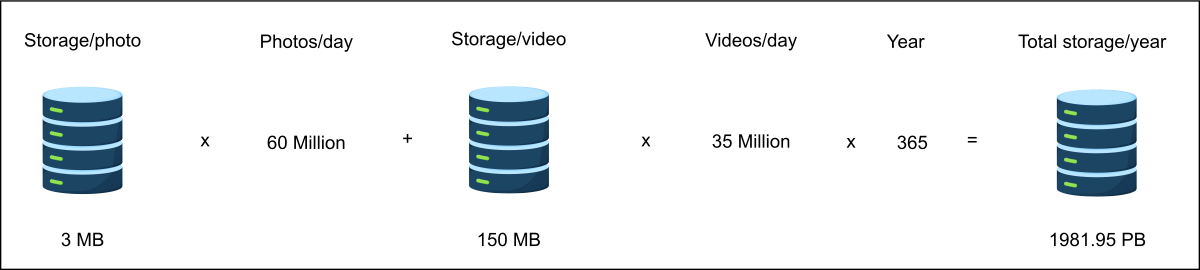
\includegraphics[width=0.5\textwidth]{Images/chapter_33/section_5571545748996096/5230795893899264.png}
 \caption{Total storage required by the Instagram storage system for a year}
\end{figure}

Besides photos and videos, we have ignored comments, status sharing data, and so on. Moreover , we also have to store users' information and post metadata, for example, userID, photo, and so on. So
, to be precise, we need more than 5430 TB/day, but to keep our design simple, let's stick to the 5430 TB/day.

\subsubsection{Bandwidth estimation}\label{ypKnXhZ-w-GYgIkUlozpY}
\\
According to the estimate of our storage capacity, our service will get 5430 TB of data each day, which will give us:
\\
\protect\phantomsection\label{katex_inline_AA0wVOJaFpXaiE5ZGl4yJ}{{{\(\frac{\text{5430 TB}}{\text{24} \times \text{60} \times \text{60}} = \frac{\text{5430 TB}}{\text{86400 sec}} \approx \text{62.84 GB/s} \approx \text{502.8 Gbps}\)}}}
\\
Since each incoming photo and video needs to reach the users' followers, let's say the ratio of readers to writers is \protect\phantomsection\label{katex_inline_y2CVsRCFf0NfvsTJ5o8NA}{{{\(100:1\)}}}. As a result, we need 100 times more outgoing bandwidth than incoming bandwidth. Let's assume the following:
\\
Incoming bandwidth \textasciitilde= 502.8 Gbps
\\
Required outgoing bandwidth \textasciitilde= \protect\phantomsection\label{katex_inline_pRZlXcdHBXuCgNYs7SZ32}{{{\(\text{100} \times \text{502.8 Gbps} \approx \text{50.28 Tbps}\)}}}

\begin{figure}[htbp]
 \centering
 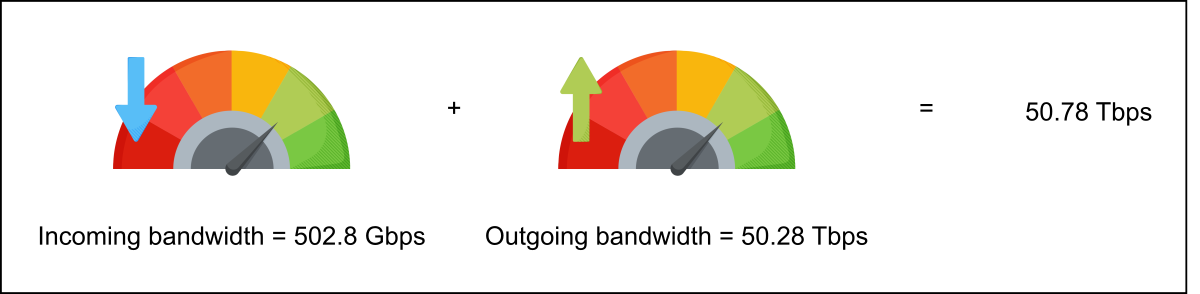
\includegraphics[width=0.5\textwidth]{Images/chapter_33/section_5571545748996096/4881092308238336.png}
 \caption{Total bandwidth required}
\end{figure}

Outgoing bandwidth is fairly high. We can use compression to reduce the media size substantially. Moreover , we'll place content close to the users via CDN and other caches in IXP and ISPs to serve the content at high speed and low latency.

\subsubsection{Server count}\label{moBBT8ya1_eDbYpcKaA3r}
\\
We will estimate server count in two ways: assuming a uniform request distribution and for the peak load. In the first method, we will assume that all the requests are distributed uniformly over a day. In some sense, that might be considered the best case for our service because the load will be ideally distributed. In the second method, we assume that all the requests of a day show up simultaneously. Such a calculation gives us an upper bound on the number of servers.
\\
One can argue that both ways might be far from the reality. However, these calculations give us lower and upper bounds on the server estimates. We can tighten these bounds by changing our assumptions. For example, if we know (or our interviewer tells us) that no more than 20\% of the daily requests can show up simultaneously, then peak server estimates will change accordingly.
\\
\paragraph{Server count assuming uniform request distribution}\label{ObDXiQXYAFkznXZCNa5uy}
\\
We need to handle concurrent requests from 500 million daily active users, which are uniformly distributed over 24 hours. Let 's assume that a typical Instagram server handles 64,000 requests per second.

\begin{itemize}
\item
\protect\phantomsection\label{2rAg_yH5QwQVyWID2pGcJ}
Requests by each user per day = \protect\phantomsection\label{katex_inline_b6WC7lXne4pZLSttBVxmF}{{{\(20\)}}}
\item
\protect\phantomsection\label{DXllna6_coBoVkFL7Wo9z}
Total requests per day = \protect\phantomsection\label{katex_inline_vzk1bEDWZFSGhv0J73wPh}{{{\(\text{500 million} \times \text{20}\)}}}
\item
\protect\phantomsection\label{Qt8qiVXQ40GICadZu8f72}
Requests per second = \protect\phantomsection\label{katex_inline_1p8XWC_LJ8UVbf5AqEuBX}{{{\(\frac{\text{500 million} \times \text{20}}{\text{24} \times \text{60} \times \text{60}} \approx \text{116 K}\)}}}
\end{itemize}
\\
The required servers are estimated as follows:

\[
\text{Servers needed for uniform requests} = \frac{\text{Number of requests/second}}{\text{RPS of server}}
\]

\[
\text{Servers needed for uniform requests} = \frac{\text{116 K}}{\text{64,000}} \approx \text{2 servers}
\]

This calculation shows that we need only 2 servers to handle queries in our Instagram system if the request load is uniformly distributed.

\begin{figure}[htbp]
 \centering
 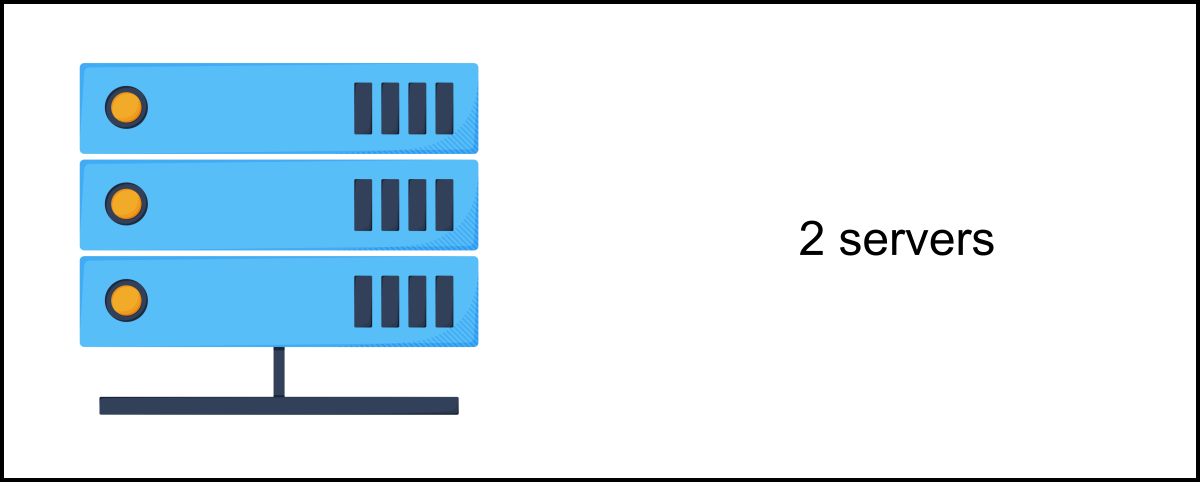
\includegraphics[width=0.15\textwidth]{Images/chapter_33/section_5571545748996096/5395675275984896.png}
 \caption{Number of servers required for the Instagram system under unifrom request distribution assumption}
\end{figure}

\paragraph{Server count assuming peak load}\label{kn4ac98QiD2zy250Tz5kz}
\\
Considering \href{https://www.educative.io/courses/grokking-the-system-design-interview/put-back-of-the-envelope-numbers-in-perspective}{our assumption} of using daily active users as a proxy for the number of requests per second to find the number of servers for peak load times, we get 500 million requests per second. Then , we use the following formula to calculate the number of servers:

\[
\text{Servers needed at peak load} = \frac{\text{Number of requests/second}}{\text{RPS of server}}
\]

\[
\text{Servers needed at peak load} = \frac{\text{500 million}}{\text{64,000}} = \text{7812.5} \approx \text{8K servers}
\]

\begin{figure}[htbp]
 \centering
 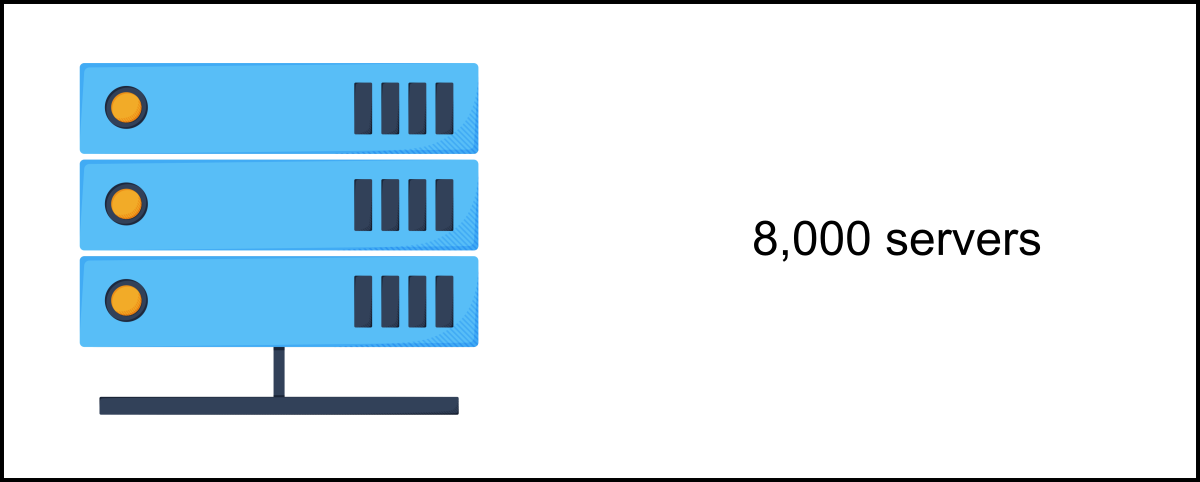
\includegraphics[width=0.15\textwidth]{Images/chapter_33/section_5571545748996096/5585832620982272.png}
 \caption{Number of servers required for the Instagram system under peak load assumption}
\end{figure}

\begin{quote}
\textbf{Note:} Concurrent requests significantly impact the number of required servers compared to requests spread over time. For a more in-depth exploration of refining peak load assumptions, refer to the ``\href{https://www.educative.io/courses/grokking-the-system-design-interview/put-back-of-the-envelope-numbers-in-perspective}{Back-of-the-envelope Calculations}'' chapter.
\end{quote}
\subsection{Try it yourself}\label{vsYJH4JW5kjtQs-scXXJc}

Let's analyze how the number of photos per day affects the storage and bandwidth requirements. For this purpose, try to change values in the following table to compute the estimates. We have set 20 requests by each user per day in the following calculation:

\subsection{Building blocks we will use}\label{WcOCoAR-_IpxyeFlwaW1y}

In the next lesson, we'll focus on the high-level design of Instagram. The design will utilize many building blocks that have been discussed in the initial chapters also. We 'll use the following building blocks in our design:

\begin{figure}[htbp]
 \centering
 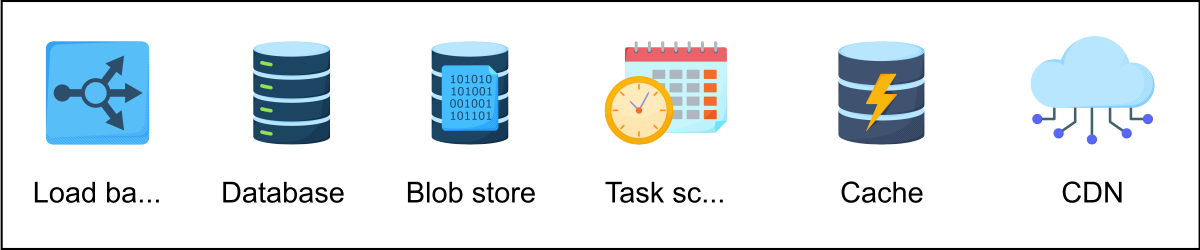
\includegraphics[width=0.5\textwidth]{Images/chapter_33/section_5571545748996096/5241138762350592.png}
 \caption{Building blocks used in Instagram design}
\end{figure}

\begin{itemize}
\item
\protect\phantomsection\label{fa0KhVnT0lVMuq61Whjzr}
A \href{https://www.educative.io/courses/grokking-the-system-design-interview/introduction-to-load-balancers}{\textbf{load balancer}} at various layers will ensure smooth request distribution among available servers.
\item
\protect\phantomsection\label{fIvHPro6Rlr4FT_YP-Tpa}
A \href{https://www.educative.io/courses/grokking-the-system-design-interview/introduction-to-databases}{\textbf{database}} is used to store the user and accounts metadata and relationship among them.
\item
\protect\phantomsection\label{xAvJ3PZB_z7GURK8smJnV}
\href{https://www.educative.io/courses/grokking-the-system-design-interview/system-design-a-blob-store}{\textbf{Blob storage}} is needed to store the various types of content such as photos, videos, and so on.
\item
\protect\phantomsection\label{BS2CBxMOvRh5LsdOJAanP}
A \href{https://www.educative.io/courses/grokking-the-system-design-interview/system-design-the-distributed-task-scheduler}{\textbf{task scheduler}} schedules the events on the database such as removing the entries whose time to live exceeds the limit.
\item
\protect\phantomsection\label{Ac4TF_B0hT9ONC4gMmu-K}
A \href{https://www.educative.io/courses/grokking-the-system-design-interview/system-design-the-distributed-cache}{\textbf{cache}} stores the most frequent content-related requests.
\item
\protect\phantomsection\label{wBvT_OOF0-5zbAwNTtLaq}
\href{https://www.educative.io/courses/grokking-the-system-design-interview/system-design-the-content-delivery-network-cdn}{\textbf{CDN}} is used to effectively deliver content to end users which reduces delay and burden on end-servers.
\end{itemize}

In the next lesson, we'll discuss the high-level design of the Instagram system.



% End of section content